\documentclass[11pt,a4paper]{article}

\usepackage[a4paper,margin=24mm]{geometry}
\usepackage{fontspec}
\usepackage{unicode-math}
\setmainfont{texgyretermes-regular.otf}[
  BoldFont=texgyretermes-bold.otf,
  ItalicFont=texgyretermes-italic.otf,
  BoldItalicFont=texgyretermes-bolditalic.otf]
\setsansfont{texgyreheros-regular.otf}[BoldFont=texgyreheros-bold.otf]
\setmonofont{lmmono10-regular.otf}[Scale=MatchLowercase]
\setmathfont{latinmodern-math.otf}
\setmathfont{latinmodern-math.otf}[version=bold,FakeBold=1.5]
\usepackage{microtype}
\usepackage{amsmath}
\usepackage{graphicx}
\usepackage{booktabs}
\usepackage{threeparttable}
\usepackage{array}
\usepackage{tabularx}
\usepackage{siunitx}
\usepackage{xcolor}
\usepackage{enumitem}
\usepackage[numbers,sort&compress]{natbib}
\usepackage[hidelinks]{hyperref}
\hypersetup{pdfauthor={Hongbai Zhu}}
\usepackage{caption}
\usepackage{subcaption}
\usepackage{placeins}

\graphicspath{{../../figures/}}
\captionsetup{font=small,labelfont=bf,labelsep=period,justification=justified,singlelinecheck=false}
\sisetup{round-mode=places,round-precision=3,detect-all}
\setlength{\parindent}{1.35em}
\setlength{\parskip}{0.20em}
\setlength{\emergencystretch}{2em}
\renewcommand{\arraystretch}{1.10}
\renewcommand{\baselinestretch}{1.06}
\newcommand{\SSCL}{\textsc{SSCL}}
\newcommand{\vect}[1]{\boldsymbol{#1}}

\title{Recovering Historical Chinese Incense Formulas under Source and Missingness Shift: A Graph Completion Benchmark with Provenance-Aware Weak Supervision}
\author{Hongbai Zhu\\[0.35em]\normalsize The Experimental High School Attached to Beijing Normal University}
\date{}

\begin{document}
\maketitle

\begin{abstract}
Historical Chinese incense books preserve formulas through compilations that differ in vocabulary, ingredient frequency, and recipe structure. We formulate restoration as weighted set completion under source shift: a model receives a known subset of a formula and predicts its hidden materials, total ingredient count, and relative composition. The data pipeline identifies 592 source-linked candidates, parses 296 ratio-ready records, and yields 237 model-facing records representing 191 provisional genealogy families. Ninety-one source-reviewed formulas from six work groups form the gold evaluation set; 146 additional records supply family-weighted weak supervision. Nested leave-one-work-out evaluation performs model and weak-label selection inside each outer training fold. A directed conditional graph raises source-macro hidden-ingredient F1 from 0.378 for global frequency to 0.426. Source-stable conditional lift reaches 0.426 and improves five work groups with one tie against frequency. EASE gives the highest weighted Jaccard, 0.473. Adding weak records leaves ingredient F1 essentially unchanged at 0.425 but reduces count mean absolute error from 1.145 to 1.089. Model ordering changes under abundance-biased, source-prefix, and unknown-fraction missingness. Nested logit calibration lowers Brier score from 0.0427 to 0.0340. A specimen-indexed chemical kernel covering 18 materials contributes no completion gain. The benchmark identifies transferable co-formulation structure, quantifies the value of automatically extracted records, and isolates material rarity as the dominant remaining error source.
\end{abstract}

\noindent\textbf{Keywords:} graph-based set completion; weak supervision; computational heritage; historical recipes; domain shift; cheminformatics

\section{Introduction}

Historical smell research has developed methods for documenting odor objects, vocabularies, places, and sensory experiences \citep{bembibre2017_smell_heritage,lisena2022_odeuropa}. Chemical analysis can reconstruct a surviving residue when a physical sample remains \citep{paolin2026_historical_smells}. Incense books often present a harder case. A formula can survive as a title, a partial ingredient list, or a later compilation, with no material sample available for chromatography or sensory testing.

Computational olfaction maps molecular structure, spectra, or controlled mixtures to perceptual descriptors \citep{keller2017_dream,gutierrez2018_semantic,lee2023_pom,sisson2025_blends}. Inverse scent design optimizes modern mixtures against a requested odor profile \citep{aleixandre2024_scent_creation}. Historical formula recovery has a different input and target. The ingredients are natural materials with variable composition, the observations are incomplete recipe records, and the source documents carry distinct editorial and compositional conventions.

This study asks which ingredient relations transfer when the target formula comes from a historical work excluded from training. We cast each formula as a sparse weighted set. The observed ingredients provide context, and the model ranks hidden materials, estimates formula size, and allocates the remaining mass. Each work group defines a source domain. The historical work is the evaluation unit because formulas in the same compilation share transmission history and terminology.

The study releases a provenance-indexed benchmark with formula genealogy and work-level splits. Source-stable conditional lift pools ingredient associations across training works and penalizes cross-work dispersion. A provenance-aware weak-supervision layer increases model-facing evidence from 91 to 237 records under target-work, target-collection, and formula-family isolation. The evaluation covers ingredient ranking, formula size, composition, probability calibration, missingness mechanisms, near-duplicate sensitivity, rare-material recovery, and computational cost. The central empirical result is a 0.048 F1 gain from conditional co-formulation over global frequency.

\section{Related Work}

\subsection{Olfactory data and inverse mixture design}

Molecular odor prediction uses physicochemical descriptors, mass spectra, learned molecular representations, and curated perceptual labels \citep{keller2017_dream,gutierrez2018_semantic,debnath2021_mass_spectra,lee2023_pom,hamel2024_pyrfume}. Blend prediction adds nonlinear interactions between odorants \citep{sisson2025_blends,thomasdanguin2014_mixtures}. These models describe molecules or controlled mixtures. Incense ingredients such as agarwood, sandalwood, resins, and processed botanicals contain many compounds whose abundance changes with taxon, plant part, preparation, and combustion. Formula completion therefore uses chemistry as supporting material evidence; it has no direct chemical measurement of the target formula.

\subsection{Missing-label learning and recommendation}

Partial formula recovery is a multi-label problem with missing positive labels. Mixed-graph multi-label methods propagate information through instance and class dependencies \citep{wu2015mlmg,zhao2018_bayesian_multilabel}. Item-based recommender models provide strong small-data comparators. EASE estimates a dense zero-diagonal item matrix by ridge regression \citep{steck2019ease}; SLIM estimates a sparse nonnegative item matrix with elastic-net regularization \citep{ning2011slim}. Nearest-neighbour and low-rank recommendation test whether formula similarity or latent structure is sufficient \citep{cover1967_nearest_neighbor,cremonesi2010_topn}.

Historical named-entity recognition addresses spelling variation, sparse annotation, and changing entity inventories \citep{sorbi2026_historical_ner}. Recipe extraction systems identify ingredients, quantities, and preparation relations in modern culinary text \citep{goel2024_recipe_ner}. Incense formula processing combines both demands: character variants must resolve to historical material identities, and quantities must link to the correct aromatic role before closure.

\subsection{Transfer and probability calibration}

Source-blocked evaluation follows the broader study of performance under distribution shift \citep{koh2021_wilds}. Cross-network transfer theory relates target error to both source performance and source-target graph discrepancy \citep{wu2023noniid}. The target work is unobserved at prediction time, so the model estimates heterogeneity among training-source conditional relations. Calibration is fitted on held-out source predictions. Temperature scaling supplies a one-parameter comparator \citep{guo2017_calibration}, and adaptive calibration error gives roughly equal-count probability groups \citep{nixon2019calibration}.

\subsection{Weak supervision for structured historical data}

Weak supervision uses programmatic rules, source metadata, and agreement patterns to enlarge training sets without assigning automatic outputs the status of expert labels \citep{ratner2017_snorkel}. Historical formula extraction provides a natural hierarchy of evidence. A source-linked candidate establishes document provenance; successful quantity parsing supplies a provisional composition; formula-family retrieval identifies copied or lightly edited witnesses; source review creates the gold label. We retain these levels instead of collapsing them into one corpus. The learning algorithm assigns less total mass to weak families and evaluates only on source-reviewed formulas.

\section{Corpus and Prediction Task}

\subsection{Reference corpus}

The corpus was assembled from public-domain Chinese incense texts and public transcriptions. Each candidate record retained the work identifier, formula title, source span, locator, material mentions, quantities, and processing notes. Aromatic masses were converted to a common relative unit and closed to sum to one. Binders, liquids, and processing aids were stored separately. Records with unresolved aromatic quantities or uncertain formula boundaries were excluded. Canonicalization preserved the source expression and mapped accepted mentions to one of 81 material identifiers. Grade terms for agarwood remained distinct.

The resulting dataset contains 91 family-unique formulas from six work groups (Table~\ref{tab:corpus}). Formula size ranges from 2 to 17 materials, with mean 6.85 and median 6. Thirty materials occur once, and four occur in more than 40 formulas. Source review accepted 91 of 120 family-deduplicated candidates, a 75.8\% release yield. The 29 exclusions record 13 quantity, 10 material-identity, eight scope, four boundary, and four role failures, with overlaps across gates. One Huizhai formula has fewer than two in-vocabulary materials in its outer training fold and is excluded from completion metrics, leaving 90 evaluated formulas. All 91 records remain part of the released corpus.

\begin{table}[t]
\centering
\caption{Historical work groups in the reference corpus. Evaluation count is the number of formulas with at least two materials represented in the corresponding outer-fold training vocabulary.}
\label{tab:corpus}
\begin{threeparttable}
\begin{tabular}{lrr}
\toprule
Work group & Corpus formulas & Evaluated formulas \\
\midrule
Chen Xiangpu compilation & 38 & 38 \\
Xiangcheng compilation & 29 & 29 \\
Huizhai Xiangpu & 10 & 9 \\
Hong Xiangpu attribution & 6 & 6 \\
Liexiang Xinpu & 6 & 6 \\
Moe Xiaolu Xiangpu & 2 & 2 \\
\midrule
Total & 91 & 90 \\
\bottomrule
\end{tabular}
\end{threeparttable}
\end{table}

\subsection{Expanded evidence corpus}

The extraction stage retains more information than the gold benchmark. It located 592 formula candidates in three public transcription collections: 332 in \emph{Xiangcheng}, 244 in \emph{Chen shi Xiangpu}, and 16 in \emph{Hong shi Xiangpu}. The parser assigned every aromatic material a mass in 296 records. These ratio-ready records contain 2 to 22 parsed aromatic materials and span 415 provisional genealogy families across the larger discovery corpus.

The V2.5 training pool separates record quality from record availability. The 91 reviewed formulas carry weight one. From the remaining ratio-ready records, 59 witnesses connected to a gold family are removed and 146 records remain eligible for weak supervision. Their 100 genealogy families combine with the 91 gold families to produce 237 model-facing records and 191 families. The weak set contains 84 \emph{Xiangcheng}, 58 \emph{Chen shi Xiangpu}, and four \emph{Hong shi Xiangpu} records. Every record retains a stable revision URL, source span, extracted ingredient mentions, original quantity strings, and normalized composition.

Figure~\ref{fig:data-scale} shows the evidence hierarchy. ``Ratio-ready'' denotes a successful deterministic parse. ``Gold'' denotes source review of formula boundary, material roles, quantities, scope, genealogy, and normalized composition. These labels enter the model through different weights and enter the evaluation through different roles.

\begin{figure}[t]
\centering
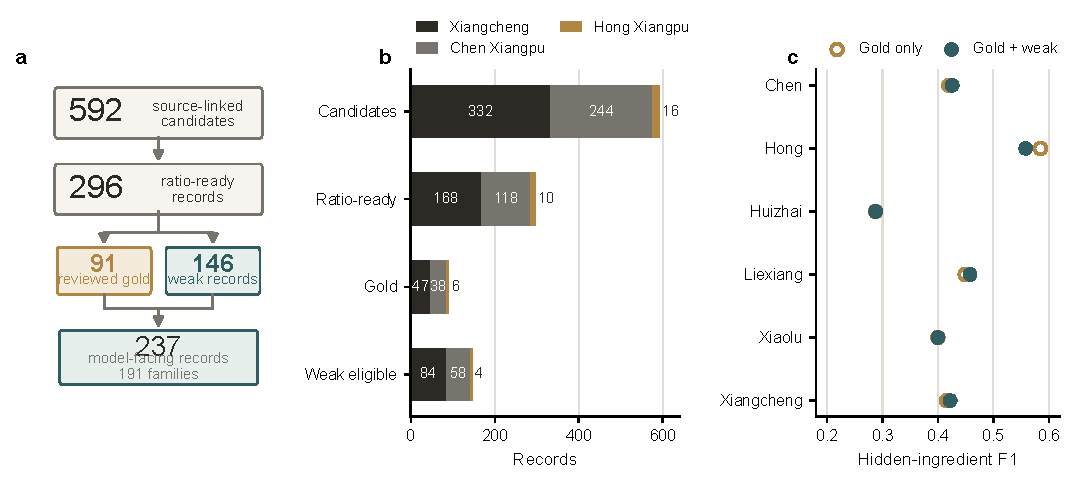
\includegraphics[width=\linewidth]{v3/v3_fig1_data_scale.pdf}
\caption{Corpus expansion and weak-supervision test. \textbf{a}, The extraction pipeline reduces 592 source-linked candidates to 296 ratio-ready records and 237 model-facing records. The final training resource contains 91 reviewed formulas and 146 weak records representing 191 genealogy families in total. \textbf{b}, Collection composition at four evidence stages. Segment labels give record counts. \textbf{c}, Work-level hidden-ingredient F1 for gold-only and weak-augmented \SSCL{}. Each point averages five masks within each evaluable gold formula and then formulas within a work. The paired work-macro change is $-0.0009$ F1, exact two-sided sign-flip $p=1.0$, $D=6$ works. Source data accompany the figure.}
\label{fig:data-scale}
\end{figure}

\begin{table}[t]
\centering
\caption{Evidence layers used in V2.5. Family count for the discovery layer refers to provisional clusters across all 592 candidates.}
\label{tab:evidence-layers}
\begin{tabularx}{\linewidth}{lrr>{\raggedright\arraybackslash}X}
\toprule
Layer & Records & Families & Model role \\
\midrule
Source-linked discovery & 592 & 415 & Candidate retrieval and coverage analysis \\
Ratio-ready extraction & 296 & 191 & Source-linked compositions available for filtering \\
Eligible weak supervision & 146 & 100 & Family-weighted training evidence \\
Reviewed reference & 91 & 91 & Unit-weight training and gold outer-fold evaluation \\
Model-facing union & 237 & 191 & Gold plus genealogy-filtered weak records \\
\bottomrule
\end{tabularx}
\end{table}

\subsection{Formula genealogy and source identity}

Formula transmission produces duplicates that ordinary record splitting cannot handle. Candidate pairs were retrieved by title bigram overlap, material-set Jaccard similarity, composition cosine similarity, and cross-witness text similarity. Connected components form provisional families. The released gold set keeps one reviewed representative per family. The weak pool excludes every family containing a gold formula, which removes 59 additional witnesses before training.

Work identity and collection identity serve different purposes. A work group marks an attributed recipe block inside a compilation and defines the inferential unit. A collection marks the public transcription source from which automatic records were extracted. When an outer fold evaluates a work, weak records from its entire collection are removed. This stronger collection block prevents unattributed records in the same compilation from re-entering training under a generic label.

\begin{figure}[t]
\centering
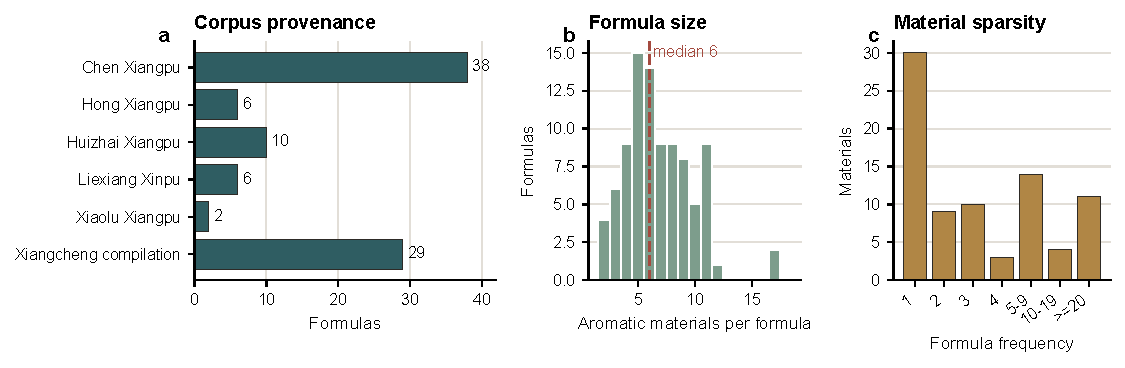
\includegraphics[width=\linewidth]{v3/v3_fig2_corpus.pdf}
\caption{Structure of the 91-formula reviewed reference set. \textbf{a}, Formula counts across six historical work groups. \textbf{b}, Distribution of aromatic materials per formula; the dashed line marks the median of six. \textbf{c}, Material-frequency distribution across the reference set. Thirty of 81 materials occur in one formula, producing a long-tailed completion target.}
\label{fig:corpus}
\end{figure}

\subsection{Weighted set representation}

For formula $i$, $q_{ij}$ is the converted aromatic mass of material $j$, and $S_i$ is its support. The closed composition follows simplex geometry \citep{aitchison1982_compositional}:
\begin{equation}
\vect{w}_i\in\Delta^{M-1},\qquad
w_{ij}=\frac{q_{ij}}{\sum_{k\in S_i}q_{ik}},\qquad
S_i=\{j:w_{ij}>0\}.
\label{eq:closure}
\end{equation}
The model receives an observed subset $O_i\subset S_i$ with its original mass fractions. It returns hidden-ingredient scores, a completed support, and a closed composition:
\begin{equation}
\mathcal{F}:\bigl(O_i,\{w_{ij}:j\in O_i\}\bigr)
\longmapsto \left(\{p_{ij}:j\notin O_i\},\widehat S_i,\widehat{\vect{w}}_i\right),
\qquad H_i=S_i\mathbin{\backslash}O_i.
\label{eq:task}
\end{equation}

\begin{table}[t]
\centering
\caption{Notation used in the model and evaluation. Every mathematical symbol in the first column is set in math mode.}
\label{tab:notation}
\small
\begin{tabularx}{\linewidth}{@{}lX@{}}
\toprule
\multicolumn{1}{c}{Symbol} & Meaning \\
\midrule
$i,j,a,b,d$ & Formula, candidate material, observed material, candidate material, and work indices \\
$S_i,O_i,H_i$ & Complete, observed, and hidden material sets for formula $i$ \\
$q_{ij},w_{ij}$ & Converted aromatic mass and closed mass fraction \\
$N_d,c_{ad},c_{abd}$ & Formula count, exposure count, and pair count within work $d$ \\
$z_i,\omega_i,\eta$ & Evidence class, formula weight, and weak-label reliability weight \\
$F(i),|F(i)|$ & Provisional genealogy family of record $i$ and its weak-record size \\
$\pi_b,\pi_{bd}$ & Global and work-specific prevalence of material $b$ \\
$\ell_{abd}$ & Conditional log-odds lift for edge $a\rightarrow b$ in work $d$ \\
$\mu_{ab},\sigma_{ab}$ & Weighted mean and standard deviation of source-specific lifts \\
$G_{ab},S_{ab}$ & Direct conditional and source-stable edge values \\
$p_{ij}$ & Candidate inclusion score or calibrated probability \\
$K_i,\widehat K_i$ & True and predicted total ingredient counts \\
$D,A_i$ & Number of outer work folds and repeated masks for formula $i$ \\
\bottomrule
\end{tabularx}
\end{table}

\subsection{Observation mechanisms}

The primary task retains half of the in-vocabulary materials. If $K_i=|S_i|$ and $f$ is the requested fraction, the observed count is
\begin{equation}
r(K_i,f)=\min\{K_i-1,\max[1,\operatorname{round}(fK_i)]\}.
\label{eq:maskcount}
\end{equation}
Five deterministic seeds select uniform subsets at $f=0.50$. Secondary tests use $f\in\{0.25,0.50,0.75\}$ and four mechanisms: uniform retention, abundance-biased retention, a prefix of the source list, and uniform retention with the decoder unaware of $f$. Hash-based seeding makes every mask reproducible.

\section{Models}

\subsection{Global and direct conditional baselines}

Let $X\in\{0,1\}^{N\times M}$ be the training presence matrix. With $c_b=\sum_i X_{ib}$, the smoothed global prevalence is
\begin{equation}
\pi_b=\frac{c_b+\tfrac12}{N+1}.
\label{eq:globalprev}
\end{equation}
The frequency baseline ranks candidates by $\pi_b$. For the directed graph, $c_a$ counts formulas containing $a$, and $c_{ab}$ counts formulas containing both $a$ and $b$. Its edge is
\begin{equation}
G_{ab}=\frac{c_{ab}+\alpha\pi_b}{c_a+\alpha},\qquad G_{aa}=1.
\label{eq:directgraph}
\end{equation}
This estimator is asymmetric because the denominators depend on the source material.

\subsection{Source-stable conditional lift}

\SSCL{} estimates the relation separately in each training work. Work prevalence shrinks toward the global prevalence:
\begin{equation}
\pi_{bd}=\frac{c_{bd}+\kappa\pi_b}{N_d+\kappa}.
\label{eq:sourceprev}
\end{equation}
For edge $a\rightarrow b$, the smoothed conditional probability is also the posterior mean under a beta prior:
\begin{align}
\theta_{abd}\mid\mathcal{D}
&\sim \operatorname{Beta}\!\left(c_{abd}+\alpha\pi_{bd},
c_{ad}-c_{abd}+\alpha(1-\pi_{bd})\right), \\
\bar\theta_{abd}
&=\mathbb{E}[\theta_{abd}\mid\mathcal{D}]
=\frac{c_{abd}+\alpha\pi_{bd}}{c_{ad}+\alpha}.
\label{eq:betaconditional}
\end{align}
Subtracting marginal log odds isolates conditional association within the work:
\begin{equation}
\ell_{abd}=\operatorname{logit}(\bar\theta_{abd})-
\operatorname{logit}(\pi_{bd}),\qquad
r_{ad}=\frac{c_{ad}}{c_{ad}+\alpha}.
\label{eq:liftweight}
\end{equation}
The exposure weight $r_{ad}$ approaches one when material $a$ has repeated support in work $d$. Across training works,
\begin{align}
\mu_{ab}&=\frac{\sum_d r_{ad}\ell_{abd}}{\sum_d r_{ad}},\\
\sigma_{ab}^{2}&=\frac{\sum_d r_{ad}(\ell_{abd}-\mu_{ab})^2}{\sum_d r_{ad}}.
\label{eq:pool}
\end{align}
The source-stable edge penalizes between-work dispersion and then blends with the direct graph:
\begin{align}
S^{\star}_{ab}&=\sigma\!\left(\beta\operatorname{logit}(\pi_b)+\mu_{ab}-\gamma\sigma_{ab}\right),\\
S_{ab}&=(1-\lambda)G_{ab}+\lambda S^{\star}_{ab}.
\label{eq:sscl}
\end{align}
Here $\sigma(x)=(1+e^{-x})^{-1}$. The dispersion term is a regularizer. Inner work folds select $\alpha$, $\gamma$, $\lambda$, and the edge reducer; $\kappa=5$ and $\beta=1$.

Given observed ingredients $O_i$, either graph supplies a candidate score through
\begin{equation}
p_{ib}=R\bigl(\{E_{ab}:a\in O_i\}\bigr),\qquad
R\in\{\operatorname{mean},\operatorname{max},\operatorname{mean\ of\ top\ 2}\},
\label{eq:reducer}
\end{equation}
where $E=G$ for the direct graph and $E=S$ for \SSCL{}.

\subsection{Provenance-aware weak supervision}

Let $z_i\in\{\mathrm{gold},\mathrm{weak}\}$ denote the evidence class and $F(i)$ the provisional genealogy family of record $i$. Gold formulas receive unit weight. Weak records share a family-level budget controlled by $\eta$:
\begin{equation}
\omega_i(\eta)=
\begin{cases}
1, & z_i=\mathrm{gold},\\[2pt]
\eta/|F(i)|, & z_i=\mathrm{weak},
\end{cases}
\qquad \eta\in\{0,0.10,0.25,0.50,1.00\}.
\label{eq:weakweight}
\end{equation}
The inverse-family term prevents a recipe with several surviving witnesses from contributing several independent formula units. Weighted sufficient statistics replace the unweighted counts:
\begin{align}
c_b^{(\omega)}&=\sum_i\omega_iX_{ib},
&c_{ab}^{(\omega)}&=\sum_i\omega_iX_{ia}X_{ib},
&N^{(\omega)}&=\sum_i\omega_i,\\
\pi_b^{(\omega)}&=\frac{c_b^{(\omega)}+\tfrac12}{N^{(\omega)}+1},
&G_{ab}^{(\omega)}&=\frac{c_{ab}^{(\omega)}+\alpha\pi_b^{(\omega)}}{c_a^{(\omega)}+\alpha}.
\label{eq:weightedstats}
\end{align}
Work-specific prevalence, lift pooling, the count histogram, EASE Gram matrix, and ratio-transfer neighbours use the same formula weights. Each weak collection enters \SSCL{} as its own source domain.

For outer target work $d^\star$, let $C(d^\star)$ be its transcription collection and $\mathcal{F}_{\mathrm{test}}$ its formula families. The admissible weak pool is
\begin{equation}
\mathcal{W}_{d^\star}=
\left\{i:z_i=\mathrm{weak},\ C(i)\ne C(d^\star),\ F(i)\notin\mathcal{F}_{\mathrm{test}}\right\}.
\label{eq:weakpool}
\end{equation}
Inner work folds apply the same rule to the inner validation work. The inner objective jointly selects $\eta$ and the structural model parameters. Values of $\eta=0$ recover gold-only training exactly.

\begin{figure}[t]
\centering
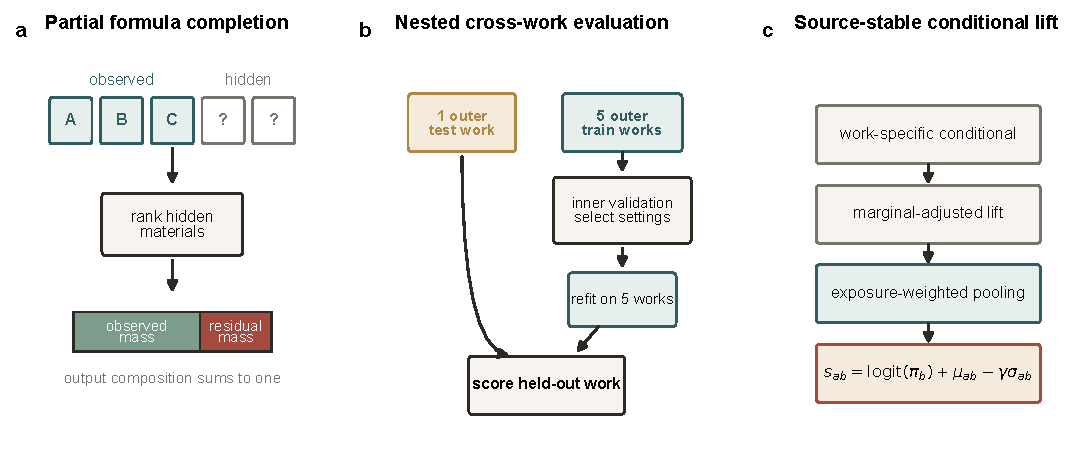
\includegraphics[width=\linewidth]{v3/v3_fig3_design.pdf}
\caption{Model and evaluation design. \textbf{a}, The model receives an observed subset with fixed masses and ranks the hidden materials before allocating residual mass. \textbf{b}, Each outer fold excludes one historical work; hyperparameters are selected by inner leave-one-work-out evaluation on the remaining works. The procedure repeats for all six targets. \textbf{c}, \SSCL{} converts work-specific conditional probabilities to marginal-adjusted lifts, pools them by exposure, and subtracts a heterogeneity penalty. The primary task uses five deterministic masks at 50\% observed context.}
\label{fig:design}
\end{figure}

\subsection{Item models and graph diffusion}

EASE learns a dense linear item matrix \citep{steck2019ease}. With $P=(X^{\top}X+\rho I)^{-1}$,
\begin{equation}
B^{\mathrm{EASE}}_{ab}=
\begin{cases}
-P_{ab}/P_{bb}, & a\ne b,\\
0, & a=b.
\end{cases}
\label{eq:ease}
\end{equation}
The SLIM-style comparator fits each candidate column with a nonnegative elastic net \citep{ning2011slim}:
\begin{equation}
\widehat B=\arg\min_{B\ge0,\,\operatorname{diag}(B)=0}
\frac{1}{2N}\lVert X-XB\rVert_F^2+
\tau\left[\eta\lVert B\rVert_1+\frac{1-\eta}{2}\lVert B\rVert_F^2\right].
\label{eq:slim}
\end{equation}
For both models, the observed binary vector multiplies $B$, followed by a small prevalence tie-breaker. Personalized graph diffusion uses the row-normalized direct graph $T$ and restart vector $u_i$:
\begin{equation}
z_i^{(t+1)}=(1-\delta)u_i+\delta z_i^{(t)}T,
\qquad z_i^{(0)}=u_i.
\label{eq:ppr}
\end{equation}
Fifty iterations produce the PPR score. Formula k-nearest neighbours and PureSVD remain secondary comparators in the stricter two-work-held-out analysis.

\subsection{Ingredient count and composition}

All ranking models share one count rule. If $n_k$ is the number of training formulas with $k$ ingredients and $K_{\max}$ is the largest training count,
\begin{equation}
p_0(K=k)=\frac{n_k+\tfrac12}{N+K_{\max}/2},\qquad
p(K=k\mid o,f)\propto p_0(K=k)\mathbf{1}\{r(k,f)=o\}\mathbf{1}\{k\ge o+1\}.
\label{eq:count}
\end{equation}
The posterior median is $\widehat K_i$. The top-ranked hidden materials fill the remaining slots. This shared module makes count error identical across ranking methods.

Observed masses remain fixed. Let $m_i=1-\sum_{a\in O_i}w_{ia}$ be residual mass and $R_{ib}$ a nonnegative ratio score obtained from the ten most similar training formulas. For selected hidden set $\widehat H_i$,
\begin{equation}
\widehat w_{ib}=
\begin{cases}
w_{ib}, & b\in O_i,\\[2pt]
m_i R_{ib}/\sum_{h\in\widehat H_i}R_{ih}, & b\in\widehat H_i,\\[2pt]
0, & \text{otherwise}.
\end{cases}
\label{eq:composition}
\end{equation}

\subsection{Nested probability calibration}

The graph scores are treated as candidate probabilities only after calibration. For each outer test work, inner held-out-work predictions fit a temperature $T$ and a two-parameter logit map:
\begin{equation}
p^{(T)}=\sigma\!\left(\frac{\operatorname{logit}(p)}{T}\right),\qquad
p^{(L)}=\sigma\!\left(a\operatorname{logit}(p)+b\right),\quad a>0.
\label{eq:calibration}
\end{equation}
Parameters minimize candidate-level negative log likelihood inside the outer training data. The outer work contributes no calibration labels.

\section{Experimental Design}

\subsection{Nested cross-work protocol}

The primary analysis uses six outer leave-one-work-out folds. The target work is absent from vocabulary construction, prevalence estimates, graph edges, and hyperparameter selection. Inside each outer training set, leave-one-work-out validation selects the configuration with highest source-macro hidden F1, using weighted Jaccard as the tie-breaker. Five mask seeds are averaged first within formula, then within work. The six work means receive equal weight.

The model grids cover direct-graph smoothing $\alpha\in\{0.5,1,2,5\}$; \SSCL{} smoothing $\alpha\in\{1,2,5\}$, penalty $\gamma\in\{0,0.25,0.5,1\}$, blend $\lambda\in\{0.25,0.5,0.75,1\}$, and mean or maximum edge reduction. EASE ridge values range from 1 to 1000. SLIM tests four penalties and three $L_1$ ratios. PPR tests five diffusion values. Five of six outer folds selected a positive \SSCL{} heterogeneity penalty.

\subsection{Weak-supervision experiment}

The data-expansion experiment repeats the full six-work outer protocol for the directed graph and \SSCL{}. Inside each outer fold, the inner work folds jointly select model parameters and $\eta$. The admissible weak pool is rebuilt for every inner and outer target. This produces 62 to 142 eligible weak records in an outer training fold, depending on which collection is blocked. Selected values of $\eta$ range from 0 to 1. The outer target contains only reviewed formulas, so the comparison measures whether automatically parsed source records improve transfer to gold formulas.

Two quantities describe weak-data exposure. The raw weak-record count measures the number of additional witnesses read by the model. The effective weak mass is
\begin{equation}
N_{\mathrm{weak}}^{\mathrm{eff}}(d)=
\sum_{i\in\mathcal{W}_d}\frac{\eta_d}{|F(i)|},
\label{eq:effectiveweak}
\end{equation}
which ranges from zero to 98.7 across the selected outer models. Ingredient ranking and count estimation can respond differently because the former depends on material-pair structure and the latter depends on the weighted formula-size histogram.

\subsection{Metrics and work-level inference}

Set recovery is measured on hidden ingredients only. For hidden truth $H_i$ and hidden prediction $\widehat H_i=\widehat S_i\mathbin{\backslash}O_i$,
\begin{align}
P_i&=\frac{|H_i\cap\widehat H_i|}{|\widehat H_i|},\qquad
R_i=\frac{|H_i\cap\widehat H_i|}{|H_i|},\qquad
F_{1i}=\frac{2P_iR_i}{P_i+R_i},\\
J_{wi}&=\frac{\sum_j\min(w_{ij},\widehat w_{ij})}
{\sum_j\max(w_{ij},\widehat w_{ij})}.
\label{eq:metrics}
\end{align}
Weighted Jaccard measures recovered composition mass. Count mean absolute error is \(|K_i-\widehat K_i|\).

For model $m$, the primary effect against frequency is the mean of paired work differences:
\begin{equation}
\widehat\Delta_m=\frac{1}{D}\sum_{d=1}^{D}
\left(\overline F_{1,md}-\overline F_{1,\mathrm{freq},d}\right),\qquad D=6.
\label{eq:estimand}
\end{equation}
An exact two-sided sign-flip test enumerates all $2^D$ work-level sign assignments:
\begin{equation}
p_{\mathrm{flip}}=2^{-D}\sum_{\vect{s}\in\{-1,1\}^{D}}
\mathbf{1}\!\left\{
\left|D^{-1}\sum_d s_d\Delta_{md}\right|\ge|\widehat\Delta_m|
\right\}.
\label{eq:signflip}
\end{equation}
The six blocks impose a coarse p-value grid. Formula masks are repeated measurements and are not treated as independent inferential units.

The primary comparison is \SSCL{} against frequency on hidden F1 in the six-work protocol. Directed graph against frequency and weak-augmented against gold-only \SSCL{} are designated secondary comparisons. The paper reports exact $p$ values and work-level effects for these comparisons. Baseline ranking, missingness, chemistry, and error analyses provide descriptive model characterization.

For calibration, Brier score and NLL are averaged first within formula and then within work. ACE is computed from candidate scores within each work. The final values are unweighted means across works. For labels $y_n\in\{0,1\}$ and probabilities $p_n$,
\begin{align}
\operatorname{Brier}&=L^{-1}\sum_{n=1}^{L}(p_n-y_n)^2,\\
\operatorname{NLL}&=-L^{-1}\sum_{n=1}^{L}\left[y_n\log p_n+(1-y_n)\log(1-p_n)\right],\\
\operatorname{ACE}&=\sum_{g=1}^{G}\frac{|I_g|}{L}
\left|\frac{1}{|I_g|}\sum_{n\in I_g}(p_n-y_n)\right|,
\label{eq:calmetrics}
\end{align}
where $I_g$ are equal-count groups within a work for ACE.

\subsection{Chemistry analysis}

The chemical registry links 18 of 81 canonical materials to specimen-level analytical profiles from 17 publications and 40 PubChem compounds. Representative sources cover agarwood, sandalwood, frankincense, clove, cassia, and cyperus \citep{ngan2020_agarwood,fatima2019_sandalwood,distefano2020_frankincense,benhassine2021_clove,firmino2018_cassia,hu2017_cyperus}. These 18 materials account for 65.24\% of aromatic-material mentions in the 296 ratio-ready records because the covered set contains recurrent bases and modifiers. Profiles retain taxon, plant part, preparation, analytical method, and measurement basis. Peak-area data, calibrated concentrations, and compound-presence reports remain separate evidence types.

For compounds $u$ and $v$ with Morgan bit sets $B_u$ and $B_v$, material-level fingerprint similarity takes the closest documented pair \citep{rogers2010_morgan}:
\begin{equation}
T_{ab}=\max_{u\in\mathcal{P}_a,\,v\in\mathcal{P}_b}
\frac{|B_u\cap B_v|}{|B_u\cup B_v|}.
\label{eq:tanimoto}
\end{equation}
Physicochemical profiles use standardized molecular weight, hydrogen-bond counts, rotatable bonds, topological polar surface area, and logP. Their material vectors are abundance-weighted compound means where numeric abundance is available and equal-weight means for presence-only profiles. Controlled odor-tag vectors use terms such as woody, balsamic, spicy, floral, camphoraceous, and animalic, with compound contributions weighted inside each profile. Cosine similarities $C^{\mathrm{phys}}$ and $C^{\mathrm{odor}}$ compare these vectors.

Morgan fingerprints, physicochemical descriptors, and controlled odor tags form three similarities. The tested kernel is
\begin{equation}
K^{\mathrm{chem}}_{ab}=\omega_f T_{ab}+
\omega_x\max(0,C^{\mathrm{phys}}_{ab})+
\omega_o\max(0,C^{\mathrm{odor}}_{ab}),\qquad
\sum_r\omega_r=1.
\label{eq:chemkernel}
\end{equation}
Development ablation and a 44-formula inverse-odor task compare the kernel with a no-chemistry model and shuffled profile assignments. The ablation applies to the 18 covered materials and their recorded profiles.

\subsection{Duplicate sensitivity, rarity, and prediction stability}

Three diagnostics examine where completion succeeds. First, a near-duplicate stress test removes every formula whose material set has Jaccard similarity at least 0.8 with a formula in another work:
\begin{equation}
J(S_i,S_r)=\frac{|S_i\cap S_r|}{|S_i\cup S_r|},
\qquad \max_{r:d_r\ne d_i}J(S_i,S_r)\ge0.8.
\label{eq:setjaccard}
\end{equation}
Second, hidden-material recall is stratified by training-fold frequency: out of vocabulary, one, two to four, and at least five appearances. Opportunity counts are pooled only for descriptive error localization. Third, prediction stability across masks is the mean pairwise Jaccard similarity among the five predicted hidden sets for each formula.

\subsection{Count intervals and case analysis}

The empirical count posterior yields a central 80\% interval $[L_i,U_i]$. A development-work-held-out conformal-style nonconformity score \citep{angelopoulos2023_conformal}
\begin{equation}
e_i=\max\{L_i-K_i,\ K_i-U_i,\ 0\}
\label{eq:countnonconformity}
\end{equation}
expands the interval by the finite-sample 0.8024 quantile of development residuals. The calibration radius is one ingredient. Coverage and mean interval width are evaluated on 1,660 repeated instances in the two-work-held-out protocol.

One formula-level analysis uses the Hong-attributed \emph{Yinxiang fa} record. The selection rule fixes seed 17 and chooses the formula closest to the six-formula median hidden F1, breaking ties by reference identifier. The example displays every observed, recovered, missed, and falsely added material together with reference and predicted mass fractions.

\subsection{Computational profile}

For $N$ formulas, vocabulary size $M$, and average formula size $\bar K$, dense graph construction costs $O(NM^2)$ if a dense presence product is formed and $O(N\bar K^2)$ when sparse hyperedges are accumulated directly. Scoring one query costs $O(|O_i|M)$ for mean or maximum reduction and $O(M\log M)$ for full sorting; partial top-$K$ selection reduces the second term to expected $O(M)$. The reference implementation uses NumPy and scikit-learn \citep{pedregosa2011_scikit} with dense arrays at $M\leq81$. Eleven repeated fits and predictions measure wall-clock time on one Apple arm64 process with data already loaded.

\section{Results}

\subsection{Conditional relations transfer across work groups}

The directed graph reached source-macro hidden F1 0.426, compared with 0.378 for frequency (Table~\ref{tab:mainresults}). It improved five work groups and tied on Xiaolu. The mean paired difference was 0.0478, and the exact two-sided sign-flip p-value was 0.0625. \SSCL{} reached F1 0.4263, a difference of 0.0481 from frequency with the same five-positive, one-tie pattern and $p=0.0625$. EASE reached F1 0.4229 and the highest weighted Jaccard, 0.4730.

\SSCL{} and the direct graph differ by 0.0003 F1, with paired $p=1.0$. Conditioning on observed ingredients accounts for the measured transfer gain; the dispersion penalty leaves aggregate performance unchanged.

\begin{table}[t]
\centering
\caption{Nested six-work formula-completion performance at 50\% uniform observation. Values are unweighted means of work-level means. Count MAE is shared because every ranking model uses the same count module.}
\label{tab:mainresults}
\begin{threeparttable}
\begin{tabular}{lSSSSS}
\toprule
Model & {Precision} & {Recall} & {Hidden F1} & {Weighted Jaccard} & {Count MAE} \\
\midrule
Frequency & 0.4323 & 0.3633 & 0.3782 & 0.4514 & 1.1447 \\
Directed graph & 0.4808 & 0.4134 & 0.4260 & 0.4699 & 1.1447 \\
\SSCL{} & 0.4802 & 0.4138 & 0.4263 & 0.4716 & 1.1447 \\
EASE & 0.4793 & 0.4082 & 0.4229 & \bfseries 0.4730 & 1.1447 \\
SLIM & 0.4402 & 0.3713 & 0.3874 & 0.4545 & 1.1447 \\
PPR & 0.4672 & 0.3968 & 0.4119 & 0.4594 & 1.1447 \\
\bottomrule
\end{tabular}
\end{threeparttable}
\end{table}

\begin{figure}[t]
\centering
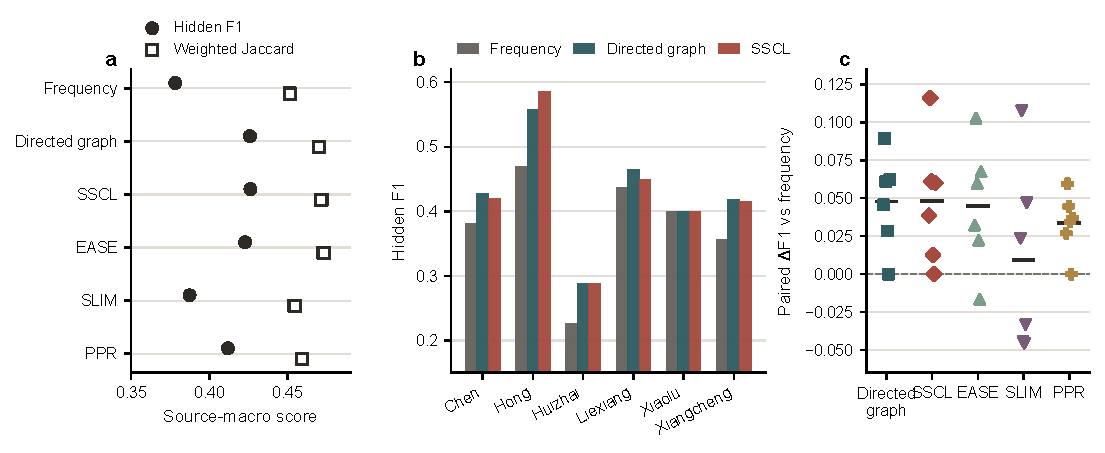
\includegraphics[width=\linewidth]{v3/v3_fig4_performance.pdf}
\caption{Nested cross-work completion performance. \textbf{a}, Source-macro hidden F1 and weighted Jaccard for six models. \textbf{b}, Work-level hidden F1 for frequency, the directed graph, and \SSCL{}. Five deterministic masks are averaged within each of 90 evaluable formulas and then within each work. \textbf{c}, Paired work-level F1 differences from frequency; points represent held-out works and horizontal bars are means. For both graph and \SSCL{}, five works improve and one ties, giving an exact two-sided sign-flip $p=0.0625$. \SSCL{} differs from the directed graph by 0.0003 F1, $p=1.0$. Source data are provided with the figure.}
\label{fig:performance}
\end{figure}

The work-level range was substantial (Table~\ref{tab:workresults}). Hong reached the highest graph scores, whereas Huizhai remained below 0.29 for every structured model. The Xiaolu estimate is based on two formulas and yields a tie among frequency, graph, and \SSCL{}. Equal work weighting keeps the large Chen and Xiangcheng groups from determining the full result.

\begin{table}[t]
\centering
\caption{Hidden F1 by held-out work. The row count gives evaluable formulas; each formula score averages five masks.}
\label{tab:workresults}
\begin{tabular}{lrrrrr}
\toprule
Work & $n$ & Frequency & Directed graph & \SSCL{} & EASE \\
\midrule
Chen & 38 & 0.3812 & 0.4268 & 0.4199 & 0.4135 \\
Hong & 6 & 0.4689 & 0.5583 & 0.5850 & 0.5717 \\
Huizhai & 9 & 0.2268 & 0.2877 & 0.2877 & 0.2867 \\
Liexiang & 6 & 0.4365 & 0.4649 & 0.4490 & 0.4588 \\
Xiaolu & 2 & 0.4000 & 0.4000 & 0.4000 & 0.3833 \\
Xiangcheng & 29 & 0.3557 & 0.4180 & 0.4159 & 0.4232 \\
\bottomrule
\end{tabular}
\end{table}

\subsection{Weak supervision expands training evidence and improves count estimation}

The ratio-ready pool increases the model-facing corpus from 91 reviewed formulas to 237 records. Depending on the blocked target collection, an outer fold admits 62 to 142 weak records from 56 to 100 families. Inner validation chooses positive weak-label weight in five of six \SSCL{} folds. The selected effective weak mass reaches 98.7 formula units when Hong is held out and 38.2 when Xiangcheng-associated work groups are held out.

Weak augmentation moves \SSCL{} hidden F1 from 0.4263 to 0.4254 (Table~\ref{tab:weakresults}), a work-macro difference of $-0.0009$ with three positive works, two ties, one negative work, and exact $p=1.0$. Directed-graph F1 moves from 0.4260 to 0.4216. Both augmented models reduce count MAE from 1.1447 to 1.0891 because the weighted formula-size histogram receives additional observations.

The work effects locate the tradeoff. Weak \SSCL{} gains 0.0060 F1 on Chen, 0.0092 on Liexiang, and 0.0062 on Xiangcheng. It loses 0.0267 on Hong and ties on Huizhai and Xiaolu. The expanded records therefore support count estimation immediately, whereas ingredient-edge quality remains controlled by source review and accurate family assignment.

\begin{table}[t]
\centering
\caption{Nested weak-supervision results. Gold-only and gold-plus-weak systems are evaluated on the same 90 gold formulas. Weak-label weight is selected inside each outer fold.}
\label{tab:weakresults}
\begin{tabular}{lSSSSS}
\toprule
Training evidence & {Precision} & {Recall} & {Hidden F1} & {Weighted Jaccard} & {Count MAE} \\
\midrule
Directed graph, gold & 0.4808 & 0.4134 & 0.4260 & 0.4699 & 1.1447 \\
Directed graph, gold + weak & 0.4725 & 0.4111 & 0.4216 & 0.4690 & 1.0891 \\
\SSCL{}, gold & 0.4802 & 0.4138 & 0.4263 & 0.4716 & 1.1447 \\
\SSCL{}, gold + weak & 0.4788 & 0.4137 & 0.4254 & 0.4704 & \bfseries 1.0891 \\
\bottomrule
\end{tabular}
\end{table}

\begin{table}[t]
\centering
\caption{Outer-fold weak-data exposure selected for \SSCL{}. Eligible weak records satisfy the collection block; effective mass is the sum of their selected sample weights.}
\label{tab:weakfolds}
\begin{tabular}{lrrrr}
\toprule
Held-out work & Gold train & Weak records & Selected $\eta$ & Effective weak mass \\
\midrule
Chen & 53 & 88 & 0.50 & 31.58 \\
Hong & 85 & 142 & 1.00 & 98.67 \\
Huizhai & 81 & 62 & 0.00 & 0.00 \\
Liexiang & 85 & 62 & 0.10 & 3.82 \\
Xiaolu & 89 & 62 & 1.00 & 38.17 \\
Xiangcheng & 62 & 62 & 1.00 & 38.17 \\
\bottomrule
\end{tabular}
\end{table}

\subsection{A stricter two-work-held-out test preserves the scale of the gain}

A secondary protocol used five development work groups, selected configurations by leave-one-work-out validation, and evaluated all ten pairs of held-out works. The direct graph reached hidden F1 0.3672 versus 0.3386 for frequency (Table~\ref{tab:hardshift}). Formula k-nearest neighbours reached 0.3431, PureSVD 0.3343, and \SSCL{} 0.3650. Weighted Jaccard favored the direct graph among V2 models and formula k-nearest neighbours across all listed comparators.

\begin{table}[t]
\centering
\caption{Secondary two-work-held-out source-shift evaluation at 50\% uniform observation.}
\label{tab:hardshift}
\begin{tabular}{lSSSS}
\toprule
Model & {Precision} & {Recall} & {Hidden F1} & {Weighted Jaccard} \\
\midrule
Frequency & 0.4054 & 0.3160 & 0.3386 & 0.4400 \\
Formula kNN & 0.4082 & 0.3233 & 0.3431 & 0.4435 \\
PureSVD & 0.3948 & 0.3161 & 0.3343 & 0.4200 \\
Directed graph & 0.4368 & 0.3437 & \bfseries 0.3672 & \bfseries 0.4494 \\
\SSCL{} & 0.4303 & 0.3451 & 0.3650 & 0.4423 \\
EASE & 0.4315 & 0.3398 & 0.3625 & 0.4450 \\
SLIM & 0.3831 & 0.3122 & 0.3273 & 0.4408 \\
PPR & 0.4315 & 0.3384 & 0.3618 & 0.4445 \\
\bottomrule
\end{tabular}
\end{table}

\subsection{Missingness mechanism changes model ordering}

At the primary 50\% context, all structured models exceeded frequency under all four observation mechanisms (Table~\ref{tab:missingness}). Their ordering changed. The directed graph led abundance-biased retention at F1 0.4295. EASE led prefix retention at 0.4812. \SSCL{} led the unknown-fraction task at 0.4038. At 75\% prefix retention, \SSCL{} reached 0.4619, compared with 0.3951 for frequency. At 75\% abundance-biased retention, frequency reached 0.3550 and exceeded the structured models.

Hidden F1 changes nonmonotonically with observed fraction because the target set changes. A larger observed subset leaves fewer hidden ingredients and can concentrate rare materials in the residual task. The uniform and unknown-fraction panels show this decline clearly.

\begin{table}[t]
\centering
\caption{Source-macro hidden F1 under four observation mechanisms at 50\% observed context.}
\label{tab:missingness}
\begin{tabular}{lrrrr}
\toprule
Mechanism & Frequency & Directed graph & \SSCL{} & EASE \\
\midrule
Uniform & 0.3782 & 0.4260 & \bfseries 0.4263 & 0.4229 \\
Abundance-biased & 0.3885 & \bfseries 0.4295 & 0.4255 & 0.4288 \\
Source-list prefix & 0.3986 & 0.4681 & 0.4662 & \bfseries 0.4812 \\
Unknown fraction & 0.3781 & 0.3920 & \bfseries 0.4038 & 0.3868 \\
\bottomrule
\end{tabular}
\end{table}

\begin{figure}[t]
\centering
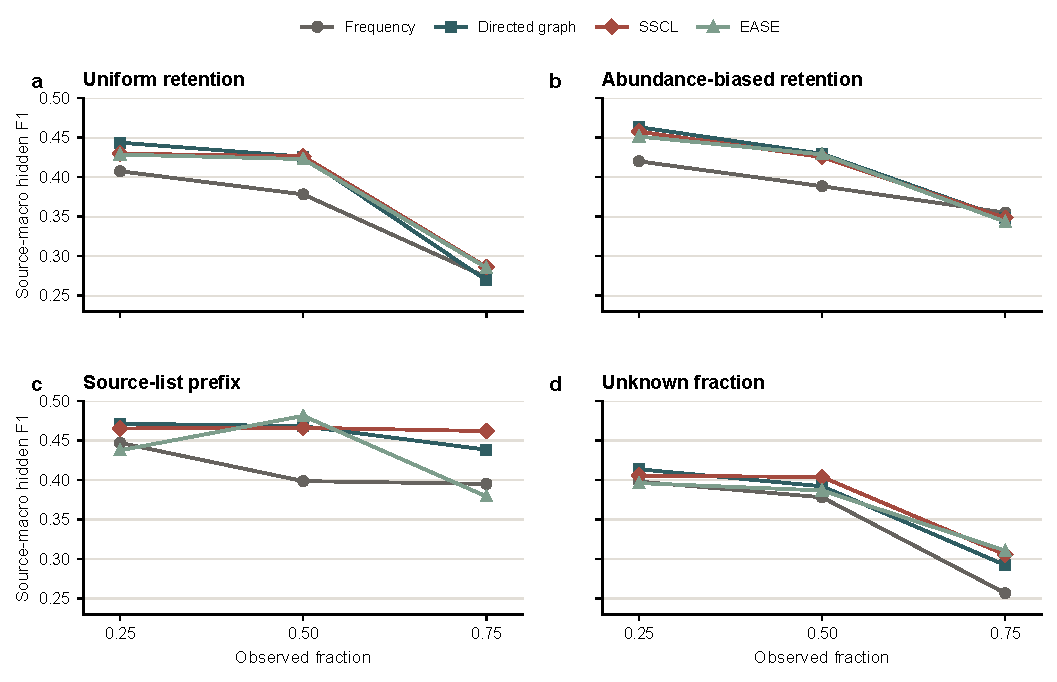
\includegraphics[width=\linewidth]{v3/v3_fig5_missingness.pdf}
\caption{Sensitivity to the observation mechanism. \textbf{a}, Uniform ingredient retention. \textbf{b}, Retention weighted by reference mass. \textbf{c}, Retention of the first ingredients in source order. \textbf{d}, Uniform retention with an unknown observed fraction in the count decoder. Points are source-macro means across six outer work folds; five deterministic masks are averaged within formula and work. Shared axes expose changes in both absolute difficulty and model ordering. Source data are provided with the figure.}
\label{fig:missingness}
\end{figure}

\subsection{Nested logit calibration removes unsupported high scores}

The uncalibrated \SSCL{} scores had source-macro Brier 0.0427, NLL 0.1572, and ACE 0.0579 (Table~\ref{tab:calibration}). Temperature scaling reduced each error. The two-parameter logit map produced Brier 0.0340, NLL 0.1262, and ACE 0.0145. Each outer calibrator was fitted exclusively on inner held-out-work predictions.

Before calibration, 186 candidate scores exceeded 0.8; their mean score was 0.839 and empirical inclusion frequency was 0.608. Logit calibration left two scores above 0.8, too few for a stable high-bin estimate. The recalibrated distribution also produced lower work-macro errors.

\begin{table}[t]
\centering
\caption{Nested calibration of \SSCL{} candidate scores. Lower Brier, NLL, and ACE values are better. The final three columns describe predictions with $p>0.8$.}
\label{tab:calibration}
\begin{tabular}{lrrrrrr}
\toprule
Method & Brier & NLL & ACE & Count & Mean $p$ & Empirical frequency \\
\midrule
Uncalibrated & 0.0427 & 0.1572 & 0.0579 & 186 & 0.839 & 0.608 \\
Temperature & 0.0406 & 0.1456 & 0.0371 & 455 & 0.874 & 0.527 \\
Logit & \bfseries 0.0340 & \bfseries 0.1262 & \bfseries 0.0145 & 2 & 0.831 & 1.000 \\
\bottomrule
\end{tabular}
\end{table}

\begin{figure}[t]
\centering
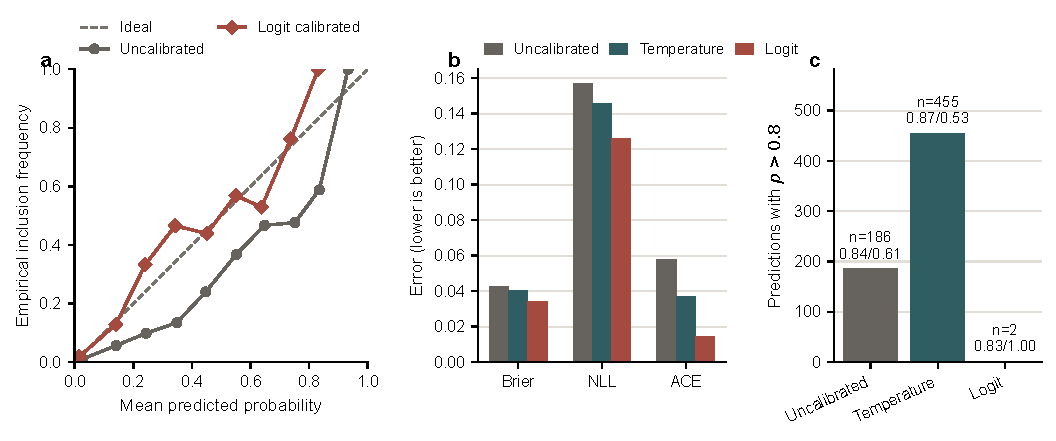
\includegraphics[width=\linewidth]{v3/v3_fig6_calibration.pdf}
\caption{Nested probability calibration. \textbf{a}, Pooled reliability bins before and after logit calibration; bin counts are available in source data. \textbf{b}, Source-macro Brier score, negative log likelihood, and adaptive calibration error. \textbf{c}, Number of predictions above 0.8; labels give count followed by mean probability and empirical inclusion frequency. Calibrators are fitted to inner held-out-work predictions for each outer fold. Two logit-calibrated predictions remain above 0.8; their empirical frequency is descriptive. Source data are provided with the figure.}
\label{fig:calibration}
\end{figure}

\subsection{Material frequency determines recoverability}

The two-work-held-out error analysis contains 6,450 hidden-material opportunities across repeated folds and masks. Materials seen at least five times in training account for 3,876 opportunities and reach recall 0.573 (Table~\ref{tab:rarity}). Recall falls to 0.056 for materials seen two to four times and 0.023 for singletons. Out-of-vocabulary materials cannot be ranked and contribute 1,445 missed opportunities. This frequency gradient explains more error than formula size: formulas with at least eight materials reach hidden F1 0.446, compared with 0.352 for formulas of size two to four and 0.344 for size five to seven.

False positives concentrate on common bases and modifiers. White sandalwood produces 462 false additions, borneol 409, musk 378, and generic agarwood 376 in the repeated two-work analysis. Frequent false negatives include scrophularia root, spikenard, zhan-grade agarwood, frankincense, and clove. The model learns productive co-formulation hubs, then overuses them when a target work applies a different convention.

\begin{table}[t]
\centering
\caption{Hidden-material recall by training-fold frequency in the two-work-held-out analysis. Opportunity counts pool ten source-pair folds and five masks and are used for error localization.}
\label{tab:rarity}
\begin{tabular}{lrrr}
\toprule
Training frequency & Recovered & Opportunities & Recall \\
\midrule
Out of vocabulary & 0 & 1,445 & 0.000 \\
One formula & 8 & 342 & 0.023 \\
Two to four formulas & 44 & 787 & 0.056 \\
At least five formulas & 2,221 & 3,876 & 0.573 \\
\bottomrule
\end{tabular}
\end{table}

\subsection{The graph advantage survives duplicate removal}

Nine formulas have cross-work material-set Jaccard similarity of at least 0.8. Removing them leaves 76 development formulas for the secondary two-work protocol. Frequency reaches hidden F1 0.3223, and the directed graph reaches 0.3482, preserving a gain of 0.0259. The earlier generalized decoder reaches 0.3494. Weighted Jaccard values are 0.3732, 0.3822, and 0.3814, respectively. The graph signal therefore persists after removing the closest cross-work analogues.

Predicted hidden sets have mean pairwise Jaccard 0.644 across the five masks. This value records genuine context dependence: changing which half of a formula is visible changes the completion, yet most selected ingredients remain shared. Figure~\ref{fig:stress} places the duplicate test beside competitive baselines and count-interval calibration from the same two-work protocol.

\begin{figure}[t]
\centering
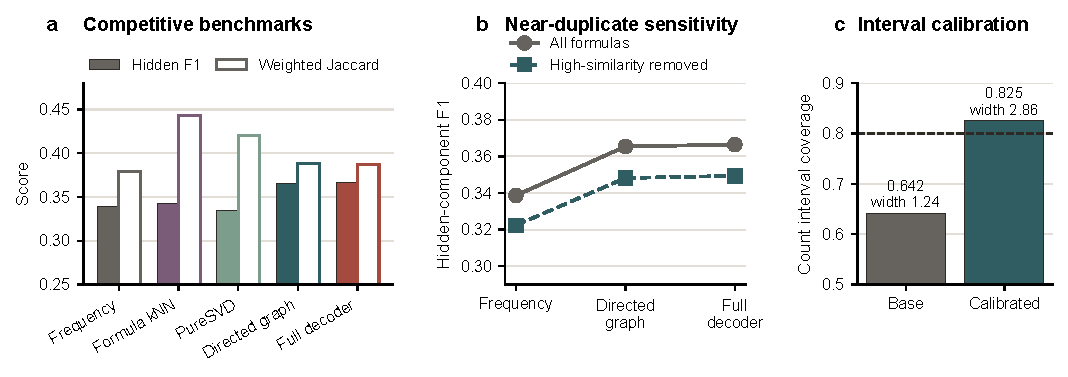
\includegraphics[width=\linewidth]{v3/v3_fig7_stress_tests.pdf}
\caption{Secondary stress tests in the two-work-held-out protocol. \textbf{a}, Hidden F1 and weighted Jaccard for frequency, formula kNN, PureSVD, the directed graph, and the earlier full decoder. Values are equal-weight means across five work groups. \textbf{b}, Hidden F1 before and after removing nine formulas with cross-work material-set Jaccard similarity at least 0.8. \textbf{c}, Coverage of central 80\% count intervals before and after development-fold residual expansion; labels give empirical coverage and mean width. The dashed line marks nominal coverage.}
\label{fig:stress}
\end{figure}

\subsection{Count calibration and residual-mass closure improve usable output}

The unexpanded central 80\% count interval covers 0.642 of 1,660 evaluation instances with mean width 1.24 ingredients. A one-ingredient development-calibrated expansion raises coverage to 0.825 with mean width 2.86. The calibration set contains 420 development-work-held-out instances, and its finite-sample quantile level is 0.8024. This interval complements the point count used in the main set-completion metric.

Composition quality depends on preserving observed evidence. In the two-work protocol, the earlier unconstrained decoder reaches source-macro weighted Jaccard 0.3871. Holding observed masses fixed and closing predicted hidden ratios to the remaining mass raises weighted Jaccard to 0.4266 without changing any selected ingredient set. Formula kNN reaches 0.4435 in the same protocol, which remains the strongest composition comparator. In the six-work V2 protocol, EASE reaches 0.4730 and \SSCL{} reaches 0.4716 with the shared residual-mass rule.

\subsection{Formula-level reconstruction reveals the error mechanism}

The \emph{Yinxiang fa} case contains 11 reference materials, six of which are observed. The model predicts the correct total count and recovers three of five hidden ingredients: zhan-grade agarwood, borneol, and white sandalwood. It misses frankincense and licorice and adds clove and linglingxiang. Hidden precision, recall, and F1 are each 0.600. The mass-constrained composition reaches weighted Jaccard 0.483.

The case shows how the graph uses conditional context. Observed agarwood, aromatic grass, musk, onycha, patchouli, and spikenard activate common wood, cooling, and spice neighbours. Borneol and sandalwood receive high inclusion scores and are recovered. Frankincense and licorice lose the ranking contest to better supported graph hubs. The predicted zhan-grade agarwood fraction is 0.117 against a reference fraction of 0.332, whereas borneol is overallocated at 0.099 against 0.013. Ingredient ranking is therefore stronger than fine-grained proportion recovery for this formula.

\begin{table}[t]
\centering
\caption{Representative \emph{Yinxiang fa} completion. Observed inputs keep their reference mass. A dash marks an unselected material.}
\label{tab:case}
\begin{tabular}{llrr}
\toprule
Material & Outcome & Reference mass & Predicted mass \\
\midrule
Agarwood & Observed & 0.066 & 0.066 \\
Aromatic grass & Observed & 0.266 & 0.266 \\
Musk & Observed & 0.053 & 0.053 \\
Onycha & Observed & 0.001 & 0.001 \\
Patchouli & Observed & 0.001 & 0.001 \\
Spikenard & Observed & 0.066 & 0.066 \\
Zhan-grade agarwood & Recovered & 0.332 & 0.117 \\
Borneol & Recovered & 0.013 & 0.099 \\
White sandalwood & Recovered & 0.066 & 0.103 \\
Frankincense & Missed & 0.066 & --- \\
Licorice & Missed & 0.066 & --- \\
Clove & Added & --- & 0.106 \\
Linglingxiang & Added & --- & 0.120 \\
\bottomrule
\end{tabular}
\end{table}

\subsection{Training and inference remain lightweight}

The earlier full probabilistic decoder, which is more expensive than the graph models used for the main V2.5 result, fits 85 formulas and 80 materials in a median 0.115 seconds over 11 runs. One prediction with 200 posterior parameter draws takes a median 1.70 milliseconds. The interquartile ranges are 0.0053 seconds for fitting and 0.14 milliseconds for prediction. Graph-only training removes logistic optimization and posterior sampling, so the reported timing supplies an upper operational reference for the current corpus scale.

\subsection{Pairwise chemistry remains neutral in completion}

The best chemistry-enabled development variant reaches hidden F1 0.3905, compared with 0.3911 for its non-chemistry counterpart, a difference of $-0.0006$. In the 44-formula inverse-odor analysis, odor kNN reaches weighted Jaccard 0.2913. The forward-consistent model reaches 0.2824, its no-chemistry ablation 0.2835, and shuffled chemical profiles 0.2863 (Table~\ref{tab:chemistry}). Pairwise material similarity is neutral for formula completion in the current representation.

The chemical registry changes the interpretation of coverage. Eighteen profiles represent 22.2\% of the 81 canonical material types and 65.24\% of aromatic-material mentions in the larger ratio-ready corpus. The recurrent materials are chemically documented; the uncovered tail is dominated by rare historical materials and unresolved botanical identities. The next chemistry model should predict interaction roles and combustion-dependent emissions through typed ingredient edges.

\begin{table}[t]
\centering
\caption{Chemistry ablations and inverse-odor composition results. Completion reports hidden F1; inverse odor reports weighted Jaccard on 44 formulas.}
\label{tab:chemistry}
\begin{tabular}{llr}
\toprule
Task & Model & Score \\
\midrule
Formula completion & No-chemistry graph decoder & 0.3911 \\
Formula completion & Chemistry-kernel decoder & 0.3905 \\
Inverse odor & Odor kNN & 0.2913 \\
Inverse odor & Forward-consistent model & 0.2824 \\
Inverse odor & No-chemistry ablation & 0.2835 \\
Inverse odor & Shuffled-profile control & 0.2863 \\
\bottomrule
\end{tabular}
\end{table}

\section{Discussion}

\subsection{Conditional co-formulation is the transferable representation}

Conditional ingredient relations raise hidden-ingredient F1 by 0.0478 over global frequency in nested six-work evaluation. The stricter two-work-held-out protocol produces a gain of 0.0286. EASE, PPR, and the directed graph all exceed frequency in the main evaluation, which places the transferable information in item dependencies. The source-stable extension reaches the same aggregate level as the direct graph. At the current number of work domains, conditional association matters more than the estimated dispersion of that association.

The result also clarifies the role of historical provenance. Formula-level random splitting mixes compilation conventions across train and test. Work-blocked evaluation measures transfer to an unseen attributed source, and collection-blocked weak supervision prevents automatic records from the target transcription from returning through an unattributed block. The reported F1 directly measures the restoration setting defined in this study.

\subsection{Weak supervision solves scale and quality as separate variables}

The new data layer increases model-facing evidence from 91 to 237 records and gives the parser a 296-record ratio-ready corpus. Ingredient F1 remains stable after weak augmentation, and count MAE falls by 0.056. These outcomes separate two effects of additional records. Formula-size statistics benefit from more examples immediately. Ingredient edges require precise material identity, formula boundaries, and genealogy because small errors are multiplied across co-occurrence pairs.

The weak-weight selections support targeted curation. Five of six outer \SSCL{} folds choose positive $\eta$, so the automatic pool contains useful structure. The strongest next data step is to review the 146 weak records in order of expected information gain. Priority goes to families that introduce a rare material into at least two source collections, reduce out-of-vocabulary opportunities in an outer fold, or create a second observation of a high-uncertainty edge. This converts the present weak pool into roughly 190 to 230 gold formulas without changing the extraction system.

\subsection{Observation process belongs inside the benchmark}

Uniform, abundance-biased, source-prefix, and unknown-fraction masks produce different model rankings. Prefix retention favors structured models because early source-listed ingredients often define a recipe base. Abundance-biased retention at 75\% leaves a small, rare residual set and allows frequency to lead. A single retention fraction cannot summarize completion quality. Reporting the observation mechanism beside the score makes the benchmark usable for damaged texts, partial transcriptions, and interactive restoration tools.

The nonmonotonic F1 curve follows directly from the changing target. At higher retention, the number of hidden items shrinks and the remaining materials shift toward the rare tail. Weighted Jaccard can still increase because more true mass is observed. Hidden F1 and weighted Jaccard therefore measure different aspects of the same completion and should remain paired.

\subsection{Probability and composition modules turn rankings into research outputs}

Logit calibration lowers work-macro Brier score by 0.0087 and ACE by 0.0434. It also removes almost all unsupported scores above 0.8. The calibrated probability answers a concrete scholarly question: how often does an ingredient with this score appear in held-out works? Count intervals provide a second uncertainty axis and reach 0.825 coverage at a nominal 0.80 after development-fold expansion.

Residual-mass closure improves composition without altering ingredient selection. The case analysis shows why composition needs its own metric: the correct hidden ingredient can receive a substantially wrong proportion. A stronger ratio module should treat formula composition as a distribution on the simplex and model ingredient-specific dispersion, processing loss, and censored quantities. Logistic-normal or Dirichlet-tree regression can use the material graph as a structured prior.

\subsection{Chemical information should model function during combustion}

The present chemical kernel measures similarity between materials. Incense formulation also depends on complementarity. A low-volatility wood can carry a volatile resin; a cooling material can balance a warm spice; a binder can change the burn rate and emission curve. The kernel omits these directed interactions, consistent with the observed $-0.0006$ F1 change.

A higher-capacity chemical layer can be built without changing the historical benchmark. Each material node can carry distributions over volatile classes, boiling points, vapor pressures, odor thresholds, and documented pyrolysis products. Edge features can encode complementary volatility ranges and shared combustion products. A message-passing network can then predict co-formulation through typed, directed interactions. Formula-linked headspace measurements would supply the strongest supervision. Published thermal-desorption and pyrolysis profiles can initialize the node features.

\section{Research Scope and Next Experiments}

The current benchmark establishes partial-formula recovery from known ingredients across six work groups. The next release will extend four dimensions.

\textbf{Corpus scale.} The 146 weak records form the immediate review queue. Reviewing them raises the gold corpus toward 237 records. Adding three further public-domain incense collections at a target of 80 to 120 accepted families each would produce 450 to 600 gold formulas and at least ten work domains. Active review will rank candidates by rare-material coverage, source novelty, and expected reduction in graph-edge variance.

\textbf{Annotation replication.} A second curator will independently annotate a stratified sample covering all works, rare materials, multi-step processing, and alternative quantities. Agreement will be reported separately for formula boundary, normalized material identity, role, quantity, and family assignment. Disagreements will create an adjudication set and a probabilistic label model for the remaining weak pool.

\textbf{Historical missingness.} Parallel witnesses and damaged recipe spans will supply empirical deletion patterns. A learned missingness model $p(O_i\mid S_i,d_i)$ can replace fixed masking and evaluate recovery under character loss, line loss, omitted quantities, and selective copying. Source-prefix masks already provide a controlled approximation for one common transmission pattern.

\textbf{Formula-to-odor bridge.} The chemistry registry will expand from 18 materials to the recurrent 40-material core, which covers most formula mentions. Published headspace, thermal-desorption, and pyrolysis data will be mapped to standardized compound identifiers and assay conditions. The resulting model will predict both hidden materials and an emission-profile distribution. Blind sensory comparison of a small, safely reproducible subset will test whether documentary completion improves perceptual similarity.

These experiments retain the same source-blocked evaluation unit. New work groups increase inferential resolution; replicated annotation measures label stability; empirical damage patterns define deployment-like inputs; combustion features connect documentary reconstruction to chemical behavior.

\section{Conclusion}

Historical incense formula recovery is a source-shifted weighted set-completion problem. Xiangji links 592 source candidates, 296 ratio-ready records, 237 model-facing formulas, and a 91-formula gold benchmark through explicit provenance and genealogy. Conditional co-formulation raises hidden-ingredient F1 from 0.378 to 0.426 across six held-out works. Weak supervision expands training evidence, improves count error, and preserves ingredient-level performance. Missingness changes model ranking, calibrated probabilities correct raw graph confidence, and material rarity explains the largest remaining error. The resulting framework joins historical text processing, graph learning, uncertainty estimation, and cheminformatics in one reproducible reconstruction task.

\section*{Data and Code Availability}

The repository contains the curated formula records, source locators, material ontology, deterministic split definitions, experiment configurations, model code, tests, figure source data, and scripts used to generate every reported result. Public release should preserve source attribution and the rights statements stored with each record.

\section*{Ethics Statement}

The study analyzes public historical texts and published chemical records. It contains no human participants, personal data, or animal experiments.

\bibliographystyle{unsrtnat}
\bibliography{xiangji_v2_5_references,xiangji_cgir_v2_methods}

\end{document}
